\subsection{Why do we want to decouple everything?}
\begin{frame}
\frametitle{Why do we want to decouple everything?}\pause
Or in other words what's wrong with monolithic systems?\pause
\begin{itemize}
	\item We can't understand a big amount of code\pause
	\item So, we can't easily add new features\pause
	\item They are complex\pause
	\item One codebase can be developed effectively by 100 people?\pause
	\item Let's skip performance and scalability
\end{itemize}
Always? It depends. The good architecture also relates to monoliths.
\end{frame}

\begin{frame}
One of the biggest advantages of distributed systems is that knowledge is
also distributed through teams. They can focus on a single part of
business requirements.

Also, It's possible to easily \textbf{replace} each part.
\end{frame}

\begin{frame}
But, everything is loosely coupled...
\end{frame}

\subsection{Architectuure!}
\begin{frame}
\frametitle{Architectuure!}
Do microservices solve your problems? ARE YOU SURE?
\begin{figure}
	\centering
	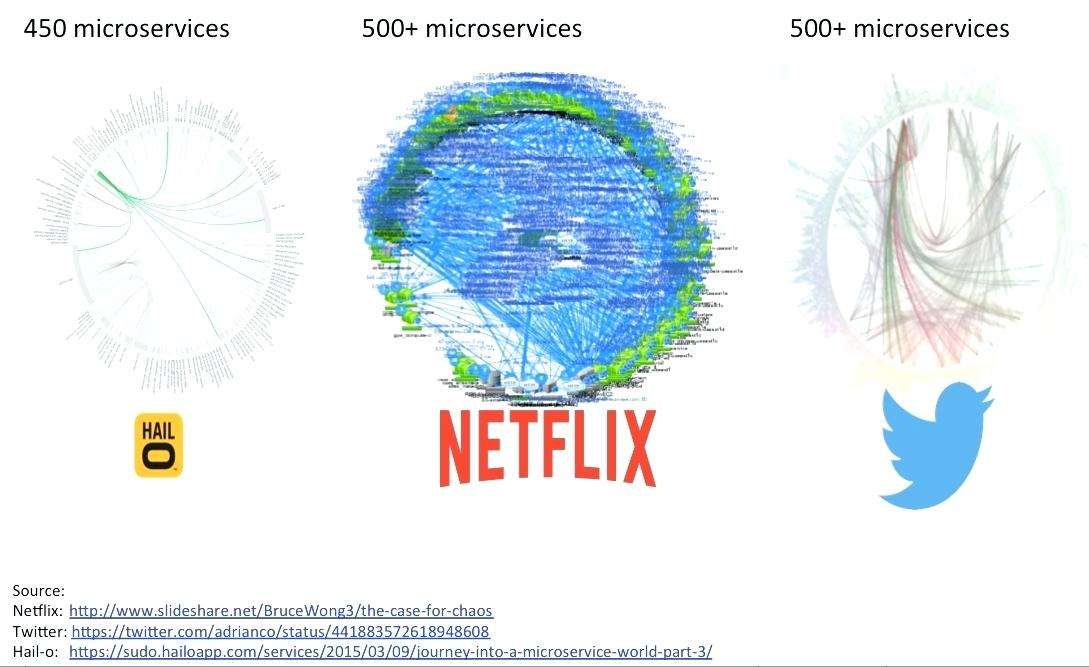
\includegraphics[width=1\linewidth]{pictures/exampleOfMicroservices}
	\label{fig:microservicesexamples}
\end{figure}


\end{frame}

\begin{frame}
\frametitle{For that - DevOps}
\begin{figure}
	\centering
	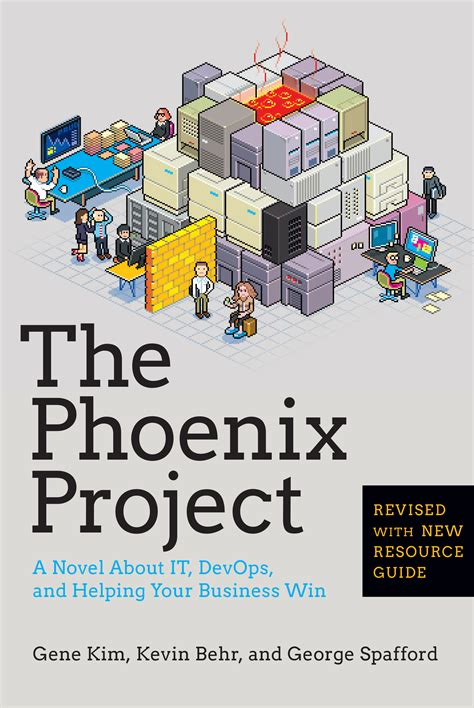
\includegraphics[width=0.4\linewidth]{pictures/fenix.jpeg}
\end{figure}


\end{frame}




\begin{frame}
\frametitle{Okay... 500 Microservices but...}
\begin{figure}
Let's connect everything on UI...\pause
\end{figure}
\begin{figure}
	\centering
	
\includegraphics[width=0.7\linewidth]{pictures/killme}
	\label{fig:killme}
\end{figure}


\end{frame}
